\newpage
{\bfseries МРНТИ 31.15.37}
\hfill {\bfseries \href{https://doi.org/10.58805/kazutb.v.2.23-442}{https://doi.org/10.58805/kazutb.v.2.23-442}}

\sectionwithauthors{O.В. Рожкова, Д.M-K. Ибраимов, В.И Рожков, М.Т. Ермеков, С.Ж.Кудайбергенова, А.Б.Букеева, Ж.Т.Нуртай}{СПОСОБ ПОЛУЧЕНИЯ СУПЕРГИДРОФОБНОЙ ГЛИНЫ МЕСТОРОЖДЕНИЯ «ТАГАНСКОЕ» ДЛЯ ПРОИЗВОДСТВА БУРОВЫХ РАСТВОРОВ}

\begin{center}
{\bfseries \textsuperscript{1,3} O.В. Рожкова\envelope, \textsuperscript{1,2}Д.M-K. Ибраимова, \textsuperscript{3,4}В.И Рожков, \textsuperscript{1}М.Т. Ермеков, \textsuperscript{3}С.Ж.Кудайбергенова, \textsuperscript{3}А.Б.Букеева, \textsuperscript{5}Ж.Т.Нуртай}

\textsuperscript{1} АО «Science and Technology Solutions», г. Алматы,
Казахстан,

\textsuperscript{2} НАО «Казахский национальный университет имени
Аль-Фараби»,

г. Алматы, Казахстан,

\textsuperscript{3} НАО \textsuperscript{«}Казахский~агротехнический
исследовательский университет им.~С.~Сейфуллина»,

г. Астана, Казахстан,

\textsuperscript{4} ТОО «Алтайский геолого-экологический институт», г.
Усть-Каменогорск, Казахстан,

\textsuperscript{5} АО «Казахский Университет технологии и бизнеса им
К.Кулажанова», г. Астана, Казахстан,

\envelope Корреспондент-автор: rozhkova.o@stsolutions.kz
\end{center}

В данной работе нами был изучен способ получения из бентонитовой глины
месторождения «Таганское» органофильной глины с краевым углом более
150°, обладающую высокой устойчивостью в органической среде, с целью
дальнейшего создания буровых растворов на ее основе, проявляющих
тиксотропные свойства в безводной среде.

В ходе проведения исследований нами был разработан новый способ
получения супергидрофобных глин из бентонитовой глины, а также изучено
их дальнейшее применение в производстве безводных буровых растворов для
нефтедобывабщей промышленности. В качестве супергидрофобизаторов нами
были использованы самые разнообразные катионные поверхностно-активные
вещества.

В присутствии тетракис(децил) бромид аммония (ТКБА) была получена
органофильная (супергидрофобная) глина с углом смачивания 170º. Было
определено распределение и устойчивость частиц органофильных глин в
дизельном топливе, полученным методом ТКБА. Доказано, что частицы
органофильной глины, полученные на основе ТКБА, образуют стабильную
суспензию в дизельном топливе и совершенно не смешиваются с водной
фазой.,

{\bfseries Ключевые слова:} супергидрофобная глина, буровой раствор,
технология, поверхностно-активные вещества, месторождение «Таганское»,
бентонит.

\begin{center}
{\large\bfseries БҰРҒЫЛАУ ЕРІТІНДІЛЕРІН ӨНДІРУ МАҚСАТЫНДА "ТАҒАН" КЕН ОРНЫНЫҢ СУПЕРГИДРОФОБТЫ САЗЫН АЛУ ТӘСІЛІ}

{\bfseries \textsuperscript{1,3} O.В. Рожкова\envelope, \textsuperscript{1,2}Д.M-K.
Ибраимова, \textsuperscript{3,4}В.И Рожков, \textsuperscript{1}М.Т.
Ермеков, \textsuperscript{3}С.Ж.Кудайбергенова,
\textsuperscript{3}А.Б.Букеева, \textsuperscript{5}Ж.Т.Нұртай}

\textsuperscript{1} «Science and Technology Solutions», АҚ, Алматы,
Қазақстан,

\textsuperscript{2} КЕАҚ «Әл-Фараби атындағы Қазақ ұлттық университеті»,
Алматы, Қазақстан,

\textsuperscript{3} КЕАҚ «С.Сейфуллин атындағы Қазақ агротехникалық
зерттеу университеті", Астана қ., Қазақстан,

\textsuperscript{4} Алтай геологиялық-экологиялық институты" ЖШС,
Өскемен қ., Қазақстан,

\textsuperscript{5} «Қ.Құлажанов атындағы Қазақ технология және бизнес
университеті» АҚ, Астана, Қазақстан

e-mail: rozhkova.o@stsolutions.kz
\end{center}

Бұл жұмыстың мақсаты - "Таған" кенорнының бентонит сазынан органикалық
ортада жоғары тұрақтылыққа ие 150° - тан асатын органофильді саз алу
әдісін, сондай-ақ, одан сусыз ортада тиксотропты қасиет көрсететін
бұрғылау ерітінділерін жасау әдісін зерттеу.

Зерттеу барысында бентонит сазынан супергидрофобты саздарды алудың жаңа
әдісін әзірленді, сонымен қатар, олардың мұнай өндіру өнеркәсібі үшін
сусыз бұрғылау ерітінділерін өндіруде одан әрі қолданылуы зерттелді.
Супергидрофобизаторлар ретінде катионды беттік активті заттардың алуан
түрін қолданылған.

Тетракис (децил) аммоний бромиді қатысында жұғу бұрышы(ТКАБ) 170º
органофильді (супергидрофобты) саз алынды. ТКАБ негізінде алынған дизель
отынындағы органофильді саз бөлшектерінің таралуы мен тұрақтылығы
анықталды. ТКБА-дан алынған органофильді саз бөлшектері дизельде тұрақты
суспензия түзетіні және су фазасымен мүлдем араласпайтыны дәлелденді.

{\bfseries Түйін сөздер:} супергидрофобты саз, бұрғылау сұйықтығы,
технология, беттік белсенді заттар, Таганское кен орны, бентонит.

\begin{center}
{\large\bfseries PRODUCING METHOD FOR SUPERHYDROPHOBIC CLAY TAGANSKOYE DEPOSIT
FOR THE DRILLING FLUIDS PRODUCTION}

{\bfseries \textsuperscript{1,3}O.V Rozhkova\envelope,
\textsuperscript{1,2}D.M-K.Ibraimova, \textsuperscript{3,4} V.I.Rozhkov,
\textsuperscript{1} M.T.Yermekov, \textsuperscript{3}S.J. Kudaibergenova,
\textsuperscript{3}A.B.Bukeeva, \textsuperscript{5}Zh.T.Nurtai}

\textsuperscript{1} SC "Science and Technology Solutions", Almaty,
Kazakhstan,

\textsuperscript{2} NC JSC "Al-Farabi Kazakh National University",

Almaty, Kazakhstan,

\textsuperscript{3} NAO "S. Seifullin Kazakh Agrotechnical Research
University", Astana, Kazakhstan,

\textsuperscript{4}Altai Geological and Ecological Institute LLP,
Ust-Kamenogorsk, Kazakhstan,

\textsuperscript{5} JSC ``Kazakh University of Technology and Business
named after K. Kulazhanov'', Astana, Kazakhstan,

e-mail: rozhkova.o@stsolutions.kz
\end{center}

In this work, we studied a method for producing organophilic clay with a
contact angle of more than 150° from bentonite clay from the Taganskoye
deposit, demonstrating high stability in an organic environment, with
the aim of further creating drilling fluids based on it, exhibiting
thixotropic properties in an anhydrous environment.

During the course of our research, A novel method for producing
superhydrophobic clays from bentonite have been developed and explored
their potential applications in the production of anhydrous drilling
fluids for the petroleum industry.

A variety of cationic surfactant compounds were used as superhydrophobic
agents.In the presence of tetrakis (decyl) ammonium bromide (TKAB),
organophilic (superhydrophobic) clay with a wetting angle of 170 degrees
was obtained. The distribution and stability of organophilic clay
particles obtained using TKAB in diesel fuel were determined. It was
proved that the particles of organophilic clay formed on the basis of
TKAB create a stable suspension in diesel fuel and do not mix with the
aqueous phase at all.

{\bfseries Keywords:} superhydrophobic clay, drilling fluid, technology,
surfactants, Taganskoye deposit, bentonite.

\begin{multicols}{2}
{\bfseries Введение.} В настоящее время, значительно возрос интерес к
бентонитовым глинам месторождения, которых встречаются на всех
континентах нашей планеты. Известно, что в природе бентониты различаются
не только по химико-минералогическому составу и физико-химическим
свойствам, но и внешним признакам. Так, интерес вызывают исследования
связанные с получением композитных глинистых материалов, в частности для
производства органомодифицированных глин (органоглин). В этой связи,
производители зачастую сталкиваются с проблемой поиска качественного
сырья для организации производства.

Ведущими мировыми производителями органоглин являются в основном
зарубежные компании, такие как Rockwood, Southern Clay Рroducts Inc.
(Cloisit, США), Sued Chemie AG (Nanofil, Германия). Для примера,
органоглина является основным наполнителем буровых растворов при бурении
нефтяных скважин, а Казахстан очень богат разнообразием глин пригодных
для их производства. Однако вследствие малоизученности этих глин, они в
настоящее время не востребованы. Несмотря на наличие достаточно обширной
информации о свойствах различных глин на территории Казахстана, имеется
лишь незначительное количество систематизированных научных работ по
возможному получению органоглин из отечественного сырья {[}1-8{]}.

В этой связи, перед нами возник интерес в проведении исследований
бентонитовой глины месторождения «Таганское» для получения органоглин
применительно к буровым растворам, поскольку они отличаются высоким
содержанием монтмориллонита, порядка 95\%. На месторождении «Таганское»
(Тарбагатайский район, Восточно-Казахстанская область, Республика
Казахстан) из-за особенностей генезиса выявлены 3 вида бентонитовой
глины: щелочной, щелочноземельный и фармацевтический, которые обладают
различными свойствами и содержанием монтмориллонита, что позволяет
использовать их в различных промышленных технологиях, в том числе и при
получении буровых растворов.

Бентонитовая глина 12-го горизонта месторождения «Таганское» на
сегодняшний день наиболее известна, так как по качественным
характеристикам она превосходит эталонный Вайомингский бентонит (США).
Ее адсорбционные свойства настолько хороши, что глина экспортируется во
Францию в качестве энтеросорбента.

Уникальность наших проводимых исследований состоит в том, что до
настоящего времени не применялись методы супергидрофобизации
монтмориллонита Таганского месторождения. Результаты ранее проведенных
нами исследований к настоящему времени приведены в статье {[}9{]} где в
качестве супергидрофобизатора использовался октадециламин и с краевым
углом смачивания 157° {[}9{]}.

Также, в некоторых работах {[}1-11{]} были проведены исследования по
получению органоглины из глин с использованием различных модификаторов,
при этом краевой угол смачивания в этих работах достигал 150°.

В данной работе, перед нами стояла задача - получить органоглину,
которая будет вводится в жидкость с очень низкой полярностью, и для
получения тиксотропных буровых растворов со стабильными свойствами
предлагается создать оптимальную органоглину. Для этого уникальная
бентонитовая глина месторождения «Таганское», из-за высокого содержания
монтмориллонита, имеет больше возможности для супергидрофобизации,
супрамолекулярной интеркаляции молекулами модификаторов.

Таким образом, целью данной работы является изучение способа получения
из монтмориллонита месторождения «Таганское» органофильной глины с
краевым углом более 150°, обладающую высокой устойчивостью в
органической среде, и предложить способ создания на его основе буровых
растворов, проявляющих тиксотропные свойства в безводной среде.

Новизна данной работы заключается в том, что нами впервые были получены
супергидрофобные органоглины на основе бентонита месторождения
«Таганское», краевой угол смачивания которых составил 170°, определена
пригодность полученной органоглины для приготовления бурового раствора и
предложены технологические схемы получения органоглины и создания
бурового раствора на их основе.

{\bfseries Материалы и методы.} В данной работе использовался
Na-монтмориллонит, полученный из бентонитовых глин месторождения
«Таганское» (карьер 12). Основой является условная химическая формула
бентонита
(OH)\textsubscript{4}Si\textsubscript{8}Al\textsubscript{4}O\textsubscript{20}·n(межпакетная)H\textsubscript{2}O.
Таганский бентонит имеет светло-розовый цвет с темно-розовыми пятнами.
Вследствие того, что в большинстве случаев существуют разные его виды,
данный тип иногда называют Таганским фармацевтическим бентонитом.

Монтмориллониты как рядовой материал не проявляют выраженной
каталитической и адсорбционной активности, поэтому их необходимо
предварительно активировать или преобразовать. Для очистки глины от
примесей ее промывали методом декантации, а затем использовали метод
термокислотной активации. Монтмориллонит сначала высушивали при
температуре 90°C в течение 2 часов, глину смешивали в соотношении 1:3 с
15\% серной кислотой, затем непрерывно перемешивали при температуре 90°C
в течение 2 часов, нагревали в растворе кислоты на водяной бане. Через 2
часа бентонит отфильтровали, поместили на фарфоровую пластину и промыли
водным раствором аммиака, затем дистиллированной водой, пока значение pH
не достигло нейтрального значения. Затем фильтрат бентонита высушивали в
лабораторной сушилке при температуре 80°C в течение. Из него получают
высушенный активированный монтмориллонит, просеивают через сито и
помещают в стеклянную коническую колбу с пришлифованной пробкой.
\end{multicols}

\begin{figure}[H]
	\centering
	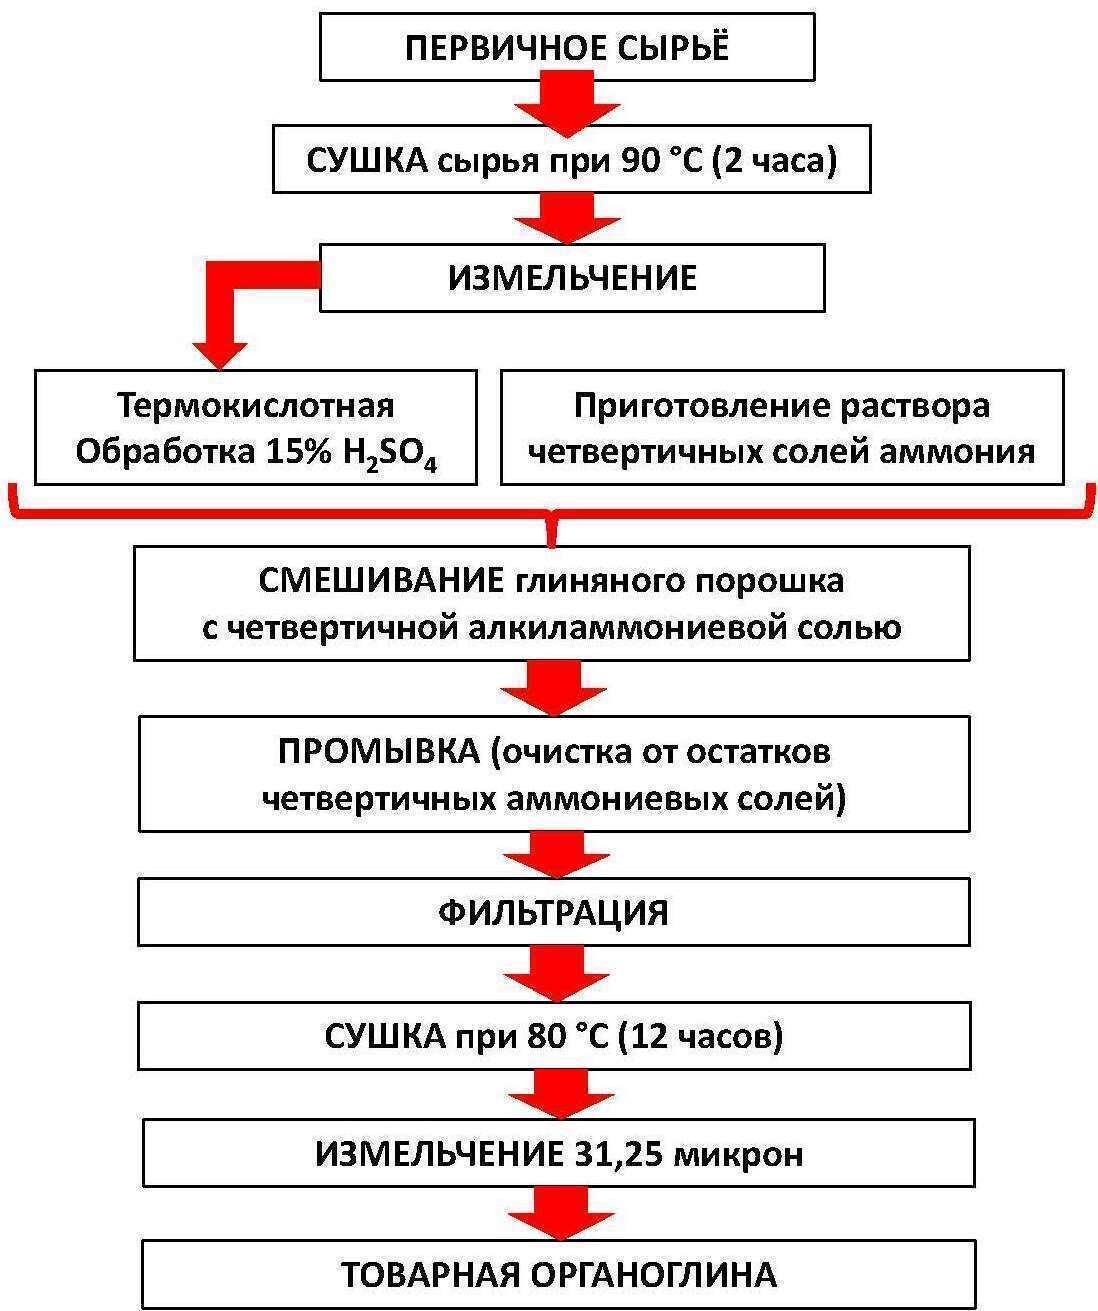
\includegraphics[width=0.6\textwidth]{assets/1014}
	\caption*{Рис. 1 -Технологическая схема производства органоглины}
\end{figure}

\begin{multicols}{2}
Рентгенодифрактометрический (XRD) метод исследования был проведен на
автоматическом дифрактометре ДРОН 3.0 с
\emph{Cu}К\emph{\textsubscript{α}}-излучением и β-фильтром. Условия
съемки дифрактограмм: U=35кВ; I=20мА; θ-2θ захват; детектор 2 град/мин.
Рентгенофазовый анализ на полуколичественной основе проводился по
дифрактограммам образцов порошка методом равных суспензий и
искусственных смесей. Было определено количественное соотношение
кристаллических фаз. Интерпретация дифрактограмм проводилась с
использованием данных из картотеки Международного центра дифракционных
данных (icdd): PDF2 порошковая дифрактометрическая база данных
(порошковая дифрактометрия) и дифрактограммы чистых от примесей
минералов. Расчет содержания проводился для основных этапов.

В качестве гидрофобизаторов для обработки Na-монтмориллонита в работе
использовались несколько поверхностно-активных веществ (ПАВ) {[}12{]}:

1) Тетракис (децил)бромид аммония (ТКБА) - C\textsubscript{40}H\textsubscript{84}BrN

2) Дидецилдиметиламмоний бромид (ДЦДMAБ) - C\textsubscript{22}H\textsubscript{48}BrN

3) Триметилоктадециламмоний бромид (ТМOДАБ)
  C\textsubscript{21}H\textsubscript{46}BrN

4) Бромид цетилпиридиния (БЦП) C\textsubscript{21}H\textsubscript{38}BrN

5) Октадециламин (ОДА) C\textsubscript{18}H\textsubscript{39}N

Реагенты, необходимые для создания буровых растворов:

В качестве органомодифицированной глины (органоглины) использовалась
супергидрофобная глина, полученная путем модификации Таганского
Na-монтмориллонита ТКБА. Обычно органоглины применяются как
структурообразующий компонент, как регулятор реологических свойств
бурового раствора, также органоглина играет роль коркообразуемого
компонента, служащего для снижения водопоглощаемости ствола скважины.

1) Приготовление растворов гидрофобизаторов и обработка глины
проводилась по следующей методике:

В процессе гидрофобизации готовили 100 мл растворов ПАВ в концентрации 1
М и 0,1 М. В приготовленные растворы помещали Na-монтмориллонитовую
глину в диапазоне 1-5 грамм и перемешивали в течение 5-6 часов в
подогреваемом лабораторном магнитной мешалке при температуре
70\textsuperscript{0} C. Порошок помещали в чашку Петри и сушили в
лабораторной сушилке до стабилизации веса, затем измельчали и просеивали
до размера 0,315 микрон. После этого определялась гидрофобность типов
органоглин.

2) Для характеристики морфологических особенностей глины использовался
метод просвечивающей электронной микроскопии {[}13{]}.

3) Гониометр ЛК-1 использовался для измерения контактного угла капли,
лежащей на поверхности порошка гидрофобной глины, по методике
стационарной лежащей неподвижной капли. Гониометр ЛК-1 создан на базе
горизонтального микроскопа и цифровой HD-видеокамеры и имеет возможности
для расчета угла контакта неподвижной капли с дисплеем {[}14{]}. Перед
определением контактных углов капель воды на поверхности гидрофобного
порошка органоглины, порошок продавливали через две стеклянные пластинки
и разглаживали.

4) Определение устойчивости супергидрофобных видов глины в средах
органических соединений. Дизельное топливо (дизтопливо) использовалось в
качестве жидкости с низкой диэлектрической проницаемостью для проверки
способности супергидрофобных глин диспергироваться в органических
средах. Приблизительная химическая формула дизтоплива: имеются
органические соединения из C\textsubscript{8}H\textsubscript{18} to
C\textsubscript{17}H\textsubscript{36}. Дизельное топливо представляет
собой сложную смесь парафиновых - предельных 10-40\% (общая формула
CnH2n+2), нафтеновых - полиметиленовых 20-60\% (общая формула CnH2n) и
ареновых - ароматических 14-30\% (общая формула CnH2n-6) углеводородов и
их производных средней молекулярной массы 110-230 г/моль, выкипающих в
пересчете на 170-380 ºC. Диэлектрическая постоянная дизтоплива
приблизительно ε=2,05 {[}15{]}.

5) Определение стабильности дисперсной среды путем осаждения в
органической среде проводилось с помощью фотоэлектрокалориметра.

6) Методы дифференциальной сканирующей калориметрии и термогравиметрии
(ДСК и ТГ) использовались для контроля влияния химических изменений в
составе органоглины под воздействием температуры, поскольку буровые
растворы могут подвергаться воздействию чрезвычайно высоких температур в
недрах земли. Эти методы проводились для изучения физико-химических и
химических процессов, происходящих в веществе при контролируемом
изменении температуры.

7) Реологические свойства буровых растворов и нефти на месторождении
Кумколь, взятых в качестве образцов, определялись простыми косвенными
методами. Например, были проведены такие измерения, как определение
плотности жидкости с помощью ареометра, определение pH раствора с
помощью pH-метра и определение вязкости с помощью реометра. Взаимосвязь
между скоростью сдвига и напряжением сдвига нефти на месторождении
Кумколь и буровых растворов на основе органоглины ТКБА определяли на
реометре MCR 702 MultiDrive (Anton Paar).

{\bfseries Результаты и обсуждение.} Глинистые минералы содержат различные
типы алюмосиликатов, основные типы которых сменяют друг друга в
природных условиях в течение миллиардов лет {[}16-18{]}. Алюмосиликатный
скелет в глинах состоит в основном из чередующихся параллельных
двумерных слоев, образованных силикатными тетраэдрами и алюминиевыми
октаэдрами {[}19-21{]}. Расположение таких слоев, степень и характер
обмена в них определяют химические и физические свойства материалов,
включая адсорбционные свойства.

Природные алюмосиликаты можно разделить на две группы в зависимости от
их кристаллической решетки - кристаллические и аморфные {[}21-22{]}.
Аморфные алюмосиликаты характеризуются способностью набухать в процессе
ионного обмена, аналогично ионообменным смолам.

На всем месторождении «Таганское» выделяют 3 вида бентонитовой глины -
щелочную (розового цвета), щелочноземельную и фармацевтическую.
Благодаря особенностям генезиса месторождения «Таганское», различные
свойства монтмориллонитов и бентонитовых глин позволяют использовать их
в различных промышленных технологических линиях. Щелочные бентониты
используются для производства буровых растворов.

С целью определения полного химического состава глины был проведен
рентгенофлуоресцентный анализ (таблица 1).
\end{multicols}


\begin{table}[H]
\caption*{Таблица 1-Оксидный химический состав бентонитовой глины месторождения «Таганское»}
\centering
\begin{tabular}{|p{0.25\textwidth}|l|l|l|l|l|l|l|p{0.1\textwidth}|}
\hline
\textbf{Содержание оксидов в минерале} & \textbf{СаO} & \textbf{MgO} & \textbf{Fe2O3} & \textbf{Al2O3} & \textbf{SiO2} & \textbf{Na2O} & \textbf{K2O} & \textbf{Остатки после сжигания} \\ \hline
Количественное соотношение оксидов в сыром минерале монтмориллоните, \% & 15 & 4 & 6 & 10 & 30 & 1,5 & 4 & 69,5 \\ \hline
Количественное соотношение оксидов в минерале Na-монтмориллонит, \% & 4 & 0,9 & 4 & 9,8 & 31 & 0,6 & 0,91 & 84,8 \\ \hline
\end{tabular}
\end{table}

\begin{multicols}{2}
Было обнаружено, что в составе бентонитовой глины наряду с элементами
Fe, Al, Si, Zn, Ti, Ca, Mn присутствует множество других элементов и
оксидов. При определении элементного состава, показано, что состав
монтмориллонита местрождения «Таганское» является кальциево-натриевым,
причиной чего является большое количество кальция.

При выполнении стадии декантационной промывки, термоактивации и
кислотной активации монтмориллонита месторождения «Таганское» удаляются
ионы кальция и магния. В результате чего увеличивается набухаемость,
ионообменная способность и межпакетное пространство глины.

С точки зрения природы монтмориллонита известно, что он
самодиспергируется в водной среде и распадается на отдельные пластинки
толщиной до 1 нм, диаметром 200-250 нм {[}23-24{]}.
\end{multicols}

\begin{figure}[H]
	\centering
	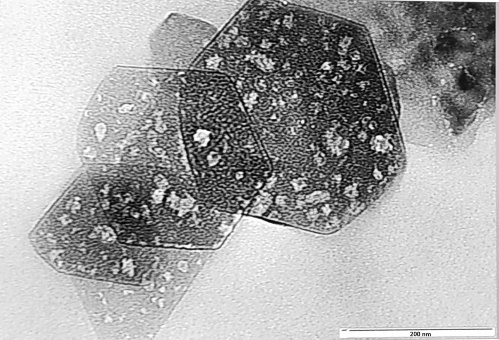
\includegraphics[width=0.5\textwidth]{assets/1015}
	\caption*{Рис. 2. - Результаты анализа методом просвечивающей электронной микроскопии монтмориллонита месторождения «Таганское»}
\end{figure}

С целью определения минерального состава бентонита месторождения
«Таганское»

и органоглины был проведен рентгенофазовый анализ. Полученные результаты
представлены в таблице 2.

\begin{table}[H]
\caption*{Таблица 2 - Минеральный состав таганского бентонита}
\centering
\begin{tabular}{|l|l|l|}
\hline
\textbf{Минерал} & \textbf{Формула} & \textbf{Количество, \%} \\ \hline
Монтмориллонит & (Na,Н)0.3(Al,Mg, Ca)2Si4O10(OH)2·xH2O & 96,4 \\ \hline
Кварц & SiO2 & 3,6 \\ \hline
\end{tabular}
\end{table}

\begin{table}[H]
\caption*{Таблица 3 - Минеральный состав органоглины, полученной с помощью ТКБА}
\centering
\begin{tabular}{|l|l|l|}
\hline
\textbf{Минерал} & \textbf{Формула} & \textbf{Количество, \%} \\ \hline
Монтмориллонит & (Na,Н)0.3(Al,Mg, Ca)2Si4O10(OH)2·xH2O & 94-97 \\ \hline
Кварц & SiO2 & 2-4 \\ \hline
Аморфная фаза & - & 1-2 \\ \hline
\end{tabular}
\end{table}

\begin{table}[H]
\caption*{Таблица 4- Контактные углы капель воды, применяемых на поверхности различных типов органомодифицированных глинопорошков}
\centering
\begin{tabular}{|p{0.3\textwidth}|ll|l|l|}
\hline
Пространственная формула модификаторов & \multicolumn{2}{p{0.2\textwidth}|}{Концентрации модификаторов и растворов монтмориллонита} & \multicolumn{1}{p{0.15\textwidth}|}{Контактный угол для монтмориллонита с органофильным покрытием} & \multicolumn{1}{p{0.2\textwidth}|}{Изображения органоглины, в присутствии различных гидрофобизаторов} \\ \cline{2-5}
 & \multicolumn{2}{l|}{Монтмориллонит} & 31⁰ & 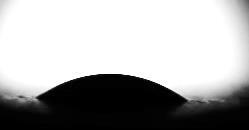
\includegraphics[height=1cm]{assets/1016} \\ \hline
\multirow{2}{*}{} & \multicolumn{1}{l|}{\multirow{2}{*}{ТМOДАБ}} & 0.1 М & 39⁰ & нет изображения \\ \cline{3-5}
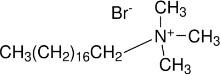
\includegraphics[width=4cm]{assets/1017} & \multicolumn{1}{l|}{} & 1 М & \textbf{9⁰} & 
\includegraphics[height=1cm]{assets/1018} \\ \hline
\multirow{2}{*}{} & \multicolumn{1}{l|}{\multirow{2}{*}{БЦП}} & 0,1М & \textbf{139⁰} & 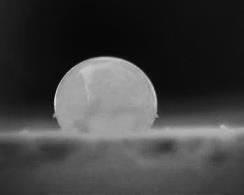
\includegraphics[height=1cm]{assets/1020} \\ \cline{3-5}
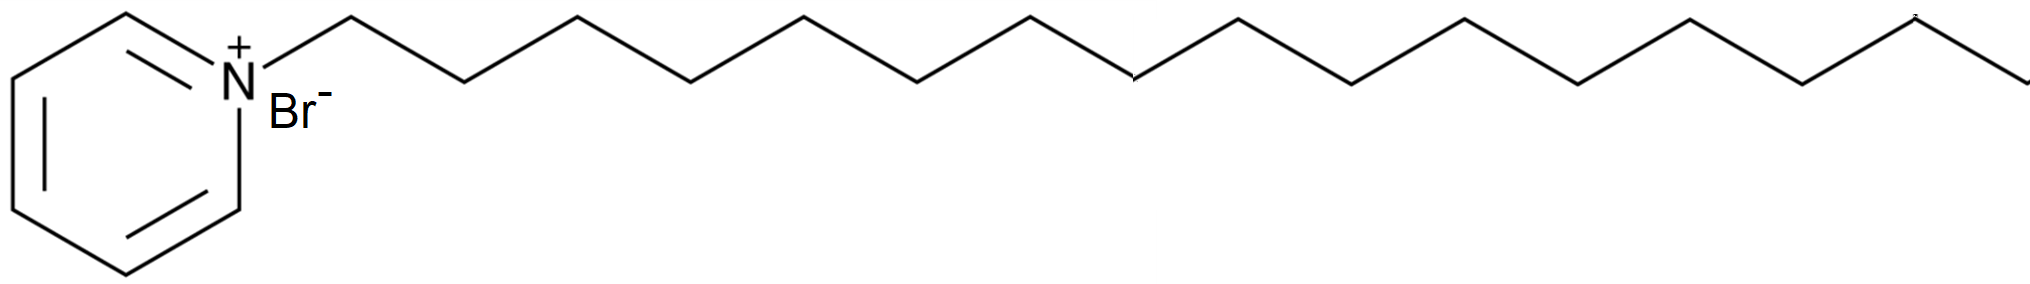
\includegraphics[width=4cm]{assets/1019} & \multicolumn{1}{l|}{} & 1 М & 128⁰ & нет изображения \\ \hline
\multirow{2}{*}{} & \multicolumn{1}{l|}{\multirow{2}{*}{ДЦДMAБ}} & 0,1М & 135⁰ & нет изображения \\ \cline{3-5}
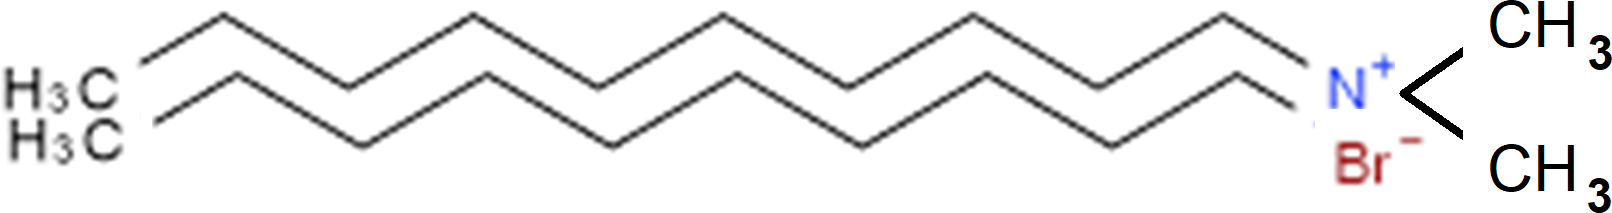
\includegraphics[width=4cm]{assets/1021} & \multicolumn{1}{l|}{} & 1 М & \textbf{161⁰} & 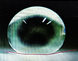
\includegraphics[height=1cm]{assets/1022} \\ \hline
\multirow{2}{*}{} & \multicolumn{1}{l|}{\multirow{2}{*}{ТКБА}} & 0,1М & 141⁰ & нет изображения \\ \cline{3-5}
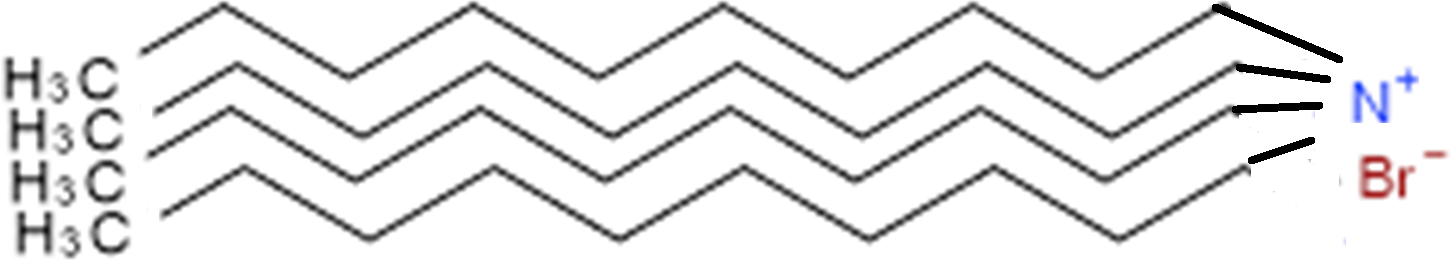
\includegraphics[width=4cm]{assets/1023} & \multicolumn{1}{l|}{} & 1 М & \textbf{170⁰} & 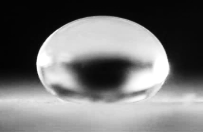
\includegraphics[height=1cm]{assets/1024} \\ \hline
\multirow{2}{*}{} & \multicolumn{1}{l|}{\multirow{2}{*}{ОДА}} & 0,1М & 131⁰ & нет изображения \\ \cline{3-5}
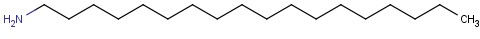
\includegraphics[width=4cm]{assets/1025} & \multicolumn{1}{l|}{} & 1 М & \textbf{157⁰} & 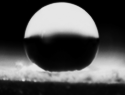
\includegraphics[height=1cm]{assets/1026} \textbf{9{]}} \\ \hline
\end{tabular}
\end{table}

\begin{multicols}{2}
В результате определения минерального состава бентонита месторождения
«Таганское» и органоглины методом рентгеноструктурного анализа было
установлено, что в составе глины, наряду с минералом монтмориллонитом,
встречаются и другие минералы в виде кварца и аморфных фаз.

В настоящее время используется несколько методов гидрофобизации
монтмориллонита. Наиболее распространенные методы гидрофобизации
монтмориллонита включают в себя методы модификации поверхности, метод
интеркаляции модификаторов и метод биогидрофобизации {[}25{]}.

Каждый из этих методов имеет как свои преимущества, так и недостатки.
Выбор того или иного метода, напраямую зависит от цели проводимого
исследования, а также от предьявляемых требований к конечному продукту
{[}26{]}. Но более подходящим и выгодным для этого направления работ
является органомодификации - метод интеркаляции, потому как, есть
необходимость учитывать кристаллическую структуру монтмориллонита.

В структурных схемах некоторые ионы
\emph{Si\textsuperscript{4}}\textsuperscript{+} обмениваются на ионы
\emph{Al\textsuperscript{3+}}. В связи с перемещением мест
\emph{Al\textsuperscript{3+}} вместо
\emph{Si\textsuperscript{4}}\textsuperscript{+} в их кристалле создается
избыточный отрицательный заряд, который компенсируется катионами
щелочных и щелочноземельных металлов, которые не связаны с определенными
местами в решетке, подвижны и могут обмениваться на другие катионы
{[}23,27-35{]}. Соответственно, глинистые частицы могут иметь
некомпенсированный отрицательный заряд на поверхности, и также при
всплытии глинистых частиц взаимодействие между аминогруппами и
глинистыми частицами может осуществляться также за счет образования
водородных связей.

Механизм адсорбции катионных ПАВ на поверхности глинистых частиц
осуществляется за счет электростатического взаимодействия. Поскольку
используемый глинистый минерал является слоистым минералом, то метод
интеркаляции эффективен как метод гидрофобизации, и основной задачей
является выбор оптимального гидрофобизатора. Далее на поверхность
различных гидрофобизаторов и обработанного порошка монтмориллонита
наносили каплю воды и измеряли значения углов смачивания этих образцов с
помощью Гониометра ЛК-1. В таблице 4 приведены значения контактных
углов, полученные для каждой из органоглин.

Среди органоглины, как указано в таблице 4, максимальный контактный угол
составил 170\textsuperscript{0} с ТКБА. Это можно объяснить структурой
молекулы ТКБА, т.е. молекула ТКБА имеет 4 длинные неполярные
углеводородные цепи, которые придают ей более гидрофобные свойства, чем
другим. Концевая сторона углеводорода ТКБА не имеет большого
пространства при плотной упаковке вместе, по сравнению с БЦП, молекула
БЦП имеет бензольное кольцо на концевой стороне, поэтому даже при самой
большой концентрации максимальное значение угла поглощения не превышало
128º.

Касательно остальных, то здесь наблюдается интересная ситуация (см.
табл. 4) при низкой концентрации гидрофобизатора (0.1 M), значения
контактных углов капель воды выше, чем при высоком значении концентрации
(1 M). В частности, в случае БЦП угол контакта уменьшился с 39º до 9º, в
случае ТМOДАБ - со 135º до 128º градусов. В других случаях, при
увеличении концентрации гидрофобизатора увеличивается и контактный угол
органоглины. Можно резюмировать, что данное снижение зависит от
особенностей этих молекул, то есть от положения и длины цепи, которую
молекула занимает на поверхности твердой частицы, что такое отклонение
произошло от слишком большой концентрации ПАВ. В результате молекула ПАВ
образует слой и происходит процесс обратной гидрофилизации поверхности
{[}36-42{]}, который показан на рис. 3:
\end{multicols}

\begin{figure}[H]
    \centering
    \begin{subfigure}[b]{0.45\textwidth}
        \centering
        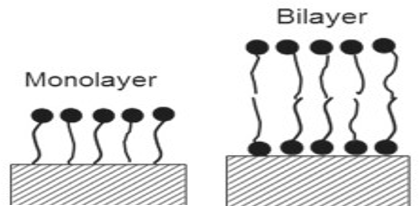
\includegraphics[width=\textwidth]{assets/1027}
        \caption*{Рис. 3 - Схематическое изображение самостоятельного взаимодействия молекул ПАВ образуя двойной слой и обратную гидрофилизации на поверхности частиц глин {[}30{]}}
    \end{subfigure}
    \hfill
    \begin{subfigure}[b]{0.45\textwidth}
        \centering
        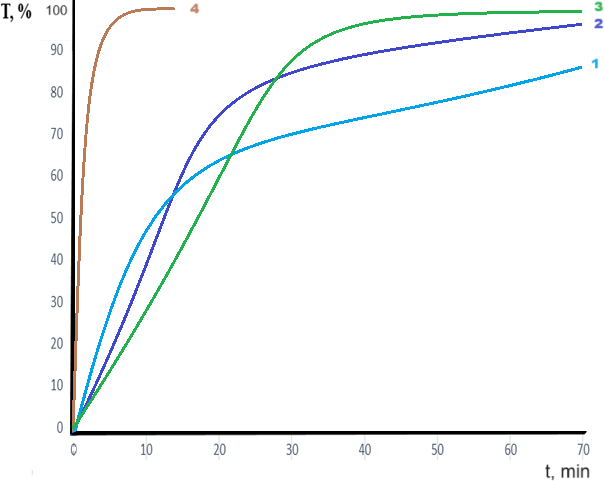
\includegraphics[width=\textwidth]{assets/1028}
        \caption*{Рис. 4 - Кинетика седиментации частиц органоглины на основе монтмориллонита в дизельном топливе, исследованная оптическим методом}
        \caption*{1-ТКБА; 2-ДЦДMAБ; 3-БЦП; 4-TOДMAБ}
    \end{subfigure}
\end{figure}

\begin{multicols}{2}
На рисунке 4 показано изменение оптически наблюдаемых значений
светопроводности суспензии органоглины, полученной с помощью различных
гидрофобизаторов, в дизтопливе в течение определенного времени.
Результаты показали, что органоглина, полученная в условиях присутствия
ТКБА, обладает наименьшим светопропусканием, а ее эквивалент составляет
82\%. В следующих исследованиях нами использовались органоглины с
наибольшим контактным углом. Было решено, что дальнейшие результаты
целесообразно продолжить с органоглиной, полученной только в присутствии
ТКБА, поскольку этот ПАВ оказался наиболее оптимальным
супергидрофобизатором.

На рисунке 5 показан результат спектрометрии на инфракрасном анализаторе
Фурье, который был получен для того, чтобы убедиться, что адсорбция ТКБА
была осуществлена на поверхности глины.
\end{multicols}

\begin{figure}[H]
    \centering
    \begin{subfigure}[b]{0.45\textwidth}
        \centering
        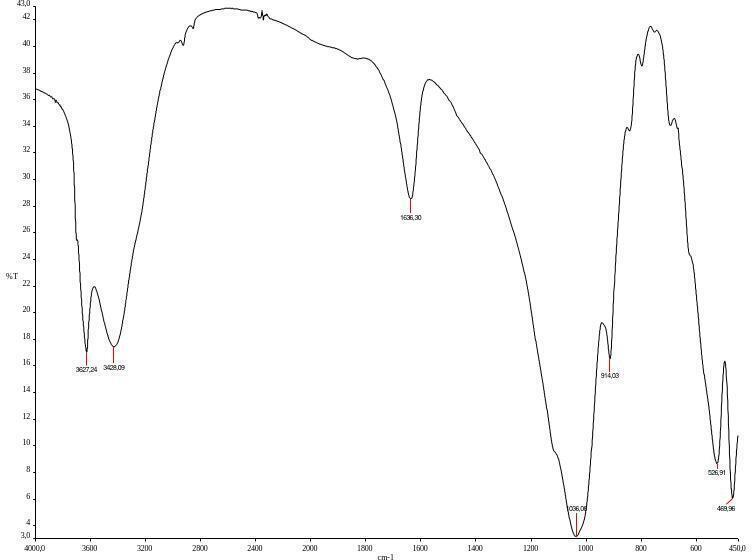
\includegraphics[width=\textwidth]{assets/1029}
        \caption*{(a)}
    \end{subfigure}
    \hfill
    \begin{subfigure}[b]{0.45\textwidth}
        \centering
        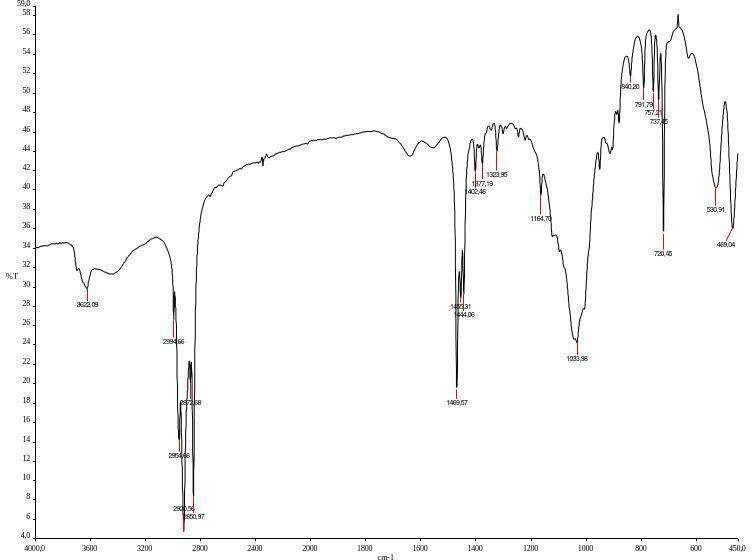
\includegraphics[width=\textwidth]{assets/1030}
        \caption*{(b)}
    \end{subfigure}
    \caption*{Рис.5 - ИК-спектры (а) Na-монтмориллонита и (б) модифицированного ТКБА органоглины}
\end{figure}

\begin{figure}[H]
	\centering
	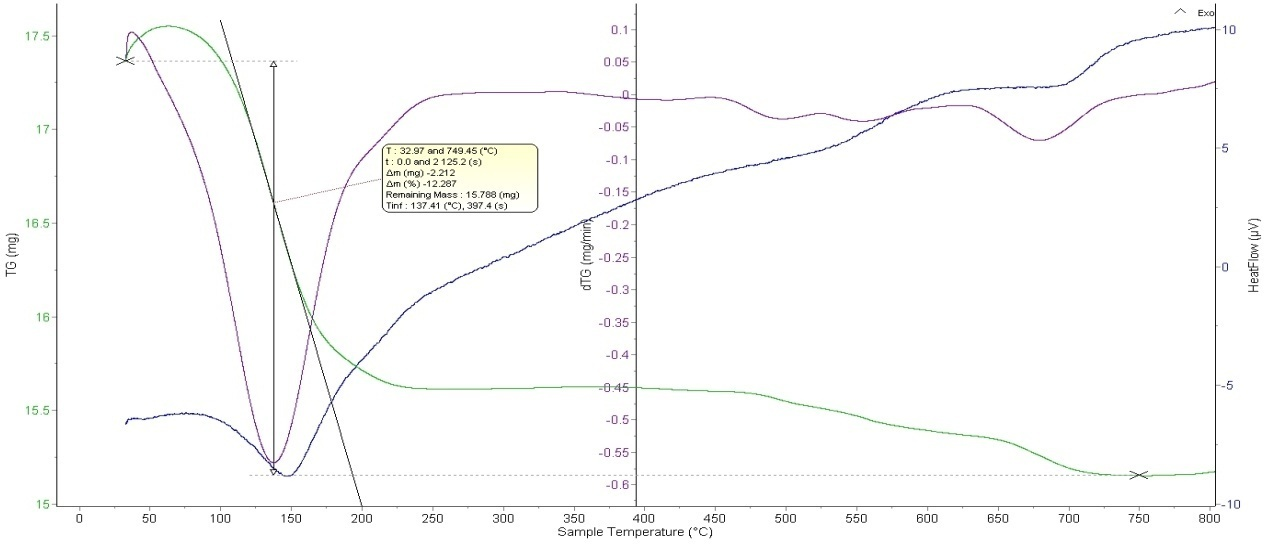
\includegraphics[width=\textwidth]{assets/1031}
	\caption*{Рис. 6. - Результаты ДСК и ТГА анализа для Na - монтмориллонита}
\end{figure}

\begin{multicols}{2}
Соответственно проведенные полосы и пики на инфракрасном анализаторе
Фурье указывают на интеркаляцию ПАВ в межслоевое пространство
монтмориллонита. В настоящее время ИК-спектроскопия является одним из
наиболее универсальных методов исследования твердого тела с помощью
компьютерных оптических методов, особенно тех, которые определяют
поверхностные группы атомов глинистого минерала и колебания элементов
его структуры, а также позволяют наблюдать изменения химических связей
при адсорбции реагентов. На рисунке 5 показаны колебания связей Si-O-Si,
наблюдаемые в широкой полосе, соответствующей 1036
см\textsuperscript{-1}. Пики по частоте 470.65 см\textsuperscript{-1} и
527 см\textsuperscript{-1} отражают колебания связи Me-O. Пики с
частотой 914 см-1 определяют колебания связей Si-О-Si. Пики в интервалах
3100-3500 см\textsuperscript{-1} (практически 3627
см\textsuperscript{-1}) молекул связаной воды в молекуле
монтмориллонита, а колебания пика при 1631 см\textsuperscript{-1}
показывают деформационные колебания, отражающие водородную связь.

В диапазоне частот 1444-1469 см\textsuperscript{-1} присутствуют пики,
которые указывают на связи C-H. Пики на 2850,97 см\textsuperscript{-1},
2954 см\textsuperscript{-1}\textsubscript{,} 2872,68
см\textsuperscript{-1}\textsubscript{,} 2994,66 см\textsuperscript{-1} и
2920,0 см\textsuperscript{-1} - показывают колебания
CH\textsubscript{2}-связей. Итак, мы убедились, что адсорбция ТКБА на
поверхности монтмориллонита происходит.

Данный анализ показывает, что при увеличении температуры от 140 ⁰ Cдо
200 ⁰ C масса исследуемого объекта уменьшается. Это показывает, что
здесь происходят различные межфазные изменения (зеленая кривая). В ходе
процесса было замечено, что при повышении температуры масса уменьшается,
то есть видно, что состав начинает отделяться от содержащегося в нем
количества воды и переходить в кристаллическую форму {[}31{]}. Было
замечено, что изменение массы замедлилось на 15,788 мг. Как мы можем
видеть, температура плавления менялась (фиолетовая кривая).
\end{multicols}

\begin{figure}[H]
	\centering
	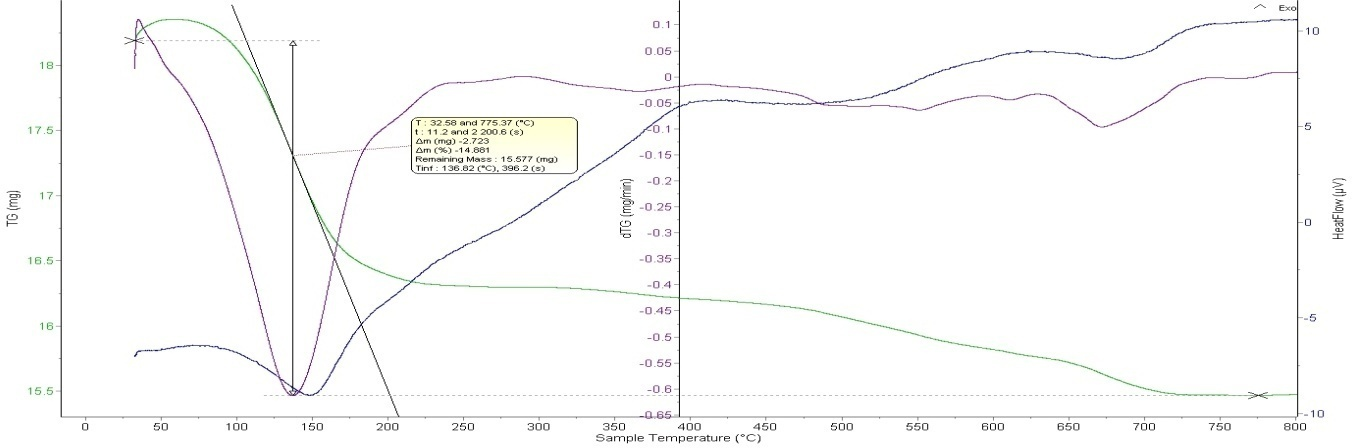
\includegraphics[width=\textwidth]{assets/1032}
	\caption*{Рис. 7- Анализ ДСК и ТГА органоглины, полученной в условиях наличия ТКБА}
\end{figure}

\begin{multicols}{2}
Наблюдаются те же явления, но потеря массы органоглины, полученной ТКБА,
происходит активнее, то есть углеводородная цепь, входящая в состав
ТКБА, окисляется в присутствии кислорода, расщепляется и улетает в виде
газа СО\textsubscript{2}. В ходе эксперимента, было замечено, что
изменение массы органоглины, полученной ТКБА замедлилось до 15 577 мг.

{\bfseries Выводы.}

1.
  Из бентонита местрождения «Таганское» Восточно-Казахстанской области
  были разработаны четыре типа органоглин при различных концентрациях
  катионных ПАВ-- 1-ТКБА; 2-ДЦДMAБ; 3-ЦПБ; 4-TOДMAБ.

2.
  Было выполнено измерение контактного угла с помощью капли воды на
  поверхности полученных органофильных глинопорошков, при этом было
  обнаружено, что при высокой концентрации ТКБА контактный угол капли
  воды равен 170º, а в присутствии других концентраций ТКБА контактный
  угол был равен всего 140º.

3.
  Изучены устойчивости органофильных глин в органической среде
  оптическим методом и самой оптимальной оказалась супергидрофобная
  глина, полученная с помощью ТКБА, мутность которой была равна 82\%.

4.
  В ходе исследований была разработана технологическая схема получения
  органоглины, был установлен способ и определена методика получения
  модифицированной органоглины с ТКБА.

\emph{{\bfseries Финансирование.} Данное научное исследование проводилось в
рамках грантового финансирования проекта ИРН AP19674742 «Технология
получения нового органоминерального композиционного материала на основе
природного бентонита Восточного Казахстана». Источник финансирования -
Комитет науки Министерства науки и высшего образования Республики
Казахстан.}

Авторы выражают благодарность за выделенное грантовое финансирование.
\end{multicols}

\begin{center}
{\bfseries Литература}
\end{center}

\begin{noparindent}
1. Ianchis R., Donescu D., Cinteza L.O.~et al\emph{.}~Polymer-clay
nanocomposites obtained by solution polymerization of vinyl benzyl
triammonium chloride in the presence of advanced functionalized clay
//J. Chem Sc.~-2014. -Vol.126. - P.609--616.
https://doi.org/10.1007/s12039-014-0621-0

2. Hodhaifa D., Meghabar R., Benachour M.~et al\emph{.}~Polymer-Clay
Nanocomposites: Exfoliation and Intercalation of Organophilic
Montmorillonite Nanofillers in Styrene--Limonene Copolymer //~Polym.
Sci. Ser\emph{. -}2021.-Vol.~63.- P.568--575.
https://doi.org/10.1134/S0965545X21050023

3. Mehri S., Ahmadinejad N., Akbarzadeh A. Vinyl Modified Cloisite 30B
Clay as an Efficient Filler for the Synthesis of
Poly(styrene-\emph{co}-butyl acrylate)/Clay Nanocomposite by Emulsion
Polymerization //Polym. Sci. Ser.- 2019.-Vol.61.-P.493-502

https://doi.org/10.1134/S1560090419040043

4. Zare Y., Fasihi M., Rhee K. Y. Efficiency of stress transfer between
polymer matrix and nanoplatelets in clay/polymer nanocomposites
//~Applied Clay Science.~ -2017. -Vol.143.-P. 265-272

https://doi.org/10.1016/j.clay.2017.03.043

5. Guanzheng Zh., Zepeng Zh., Maguy J. Organoclays used as colloidal and
rheological additives in oil-based drilling fluids: An overview//
Applied Clay Science. -2019.-Vol.177.-P.63-81,

https://doi.org/10.1016/j.clay.2019.05.006

6. Rogers K., Takács E., Thompson M. Contact angle measurement of select
compatibilizers for polymer-silicate layer nanocomposites //Polimer
Testing.-2005.-Vol.24.- P.423-427.

https://doi.org/10.1016/j.polymertesting.2005.01.010

7. Pegoretti A., Dorigato A., Brugnara M., Penati, A. Contact angle
measurements as a tool to investigate the filler--matrix interactions in
polyurethane--clay nanocomposites from blocked prepolymer// European
Polymer Journal. -2008. -Vol. 44(6). - P.1662-1672.~

https://doi.org/10.1016/j.eurpolymj.2008.04.011

8. Elias E., Chandran C. S., Chandran N., Souza F. G., Thomas
S. Segmental dynamics, morphology and

thermomechanical properties of
electrospun poly(ε-caprolactone) nanofibers in the presence of an
interacting filler // RSC Advances.-2016. -Vol.6(26).-
P.21376--21386.~https://doi.org/10.1039/c5ra24251g

9. Musabekov K.B., Artykova D.M-K., Tazhibayeva S.M., Oryntaeva A.,
Sugurbekova G.K., Kulichikhin V. Surface modification of montmorillonite
clay with organic molecules // Rasayan J. Chem.-
2021.-Vol.14(1).-P.635-640. http://dx.doi.org/10.31788/RJC.2021.1416093

10. Hadj-Hamou A.S., Metref F., Yahiaoui F. Thermal stability and
decomposition kinetic studies of antimicrobial PCL/nanoclay packaging
films //~Polym. Bull.-
2017.-Vol.74.-P.3833--3853.~https://doi.org/10.1007/s00289-017-1929-y

11. Kurmangazhi G., Tazhibayeva S. M.,~ Musabekov K. B.,~ Levin I. S.,~
Kuzin M. S.,~ Ermakova L. E.,~~Yu V. K.~ Preparation of Dispersed
Magnetite--Bentonite Composites and Kazcaine Adsorption on Them
//~Colloid J.-~2021. -Vol.83.- P.343-351.

https://doi.org/10.1134/S1061933X21030091

12.
https://www.sigmaaldrich.com/KZ/en/products/chemistry-and-biochemicals/lab-chemicals-

Date of address:12.02.2024

13. https://www.facebook.com/kjickaznau/- Date of address:12.02.2024

14. https://www.openscience.ru/chem/index.php?page=wetting\&item=003-

Date of address:16.02.2024

15. https://fundamental-research.ru/ru/article/view?id=3212- Date of
address:16.02.2024

16. Cailun W., Myshkin V.E., Bespala E.V., Poberezhnikov А.D., Baraban
А.P., Shukshina D.D., Semenov D.А. Structure and properties of
montmorillonite containing Ca\textsuperscript{2+},
Sr\textsuperscript{2+}, and Ba\textsuperscript{2+}~cations
simultaneously // Journal of Molecular Liquids. -2023. -Vol. 382. -
121994.

https://doi.org/10.1016/j.molliq.2023.121994

17.Brigatti M. F., Galan E., Theng B. K. G. Chapter 2 Structures and
Mineralogy of Clay Minerals// Developments of Clay Science. -2006.
-Vol.1.- P.9 - 86.~

https://doi.org/10.1016/s1572-4352(05)01002-0

18. Peng J., Yi H., Song S., Zhan W., Zhao Y. Driving force for the
swelling of montmorillonite as affected by surface charge and
exchangeable cations: A molecular dynamic study// Results in Physics.
-2019. -Vol.12.- P.113-117.~https://doi.org/10.1016/j.rinp.2018.11.011

19. Ngouana BFW, Kalinichev AG. Structural arrangements of isomorphic
substitutions in smectites: Molecular simulation of the swelling
properties, interlayer structure, and dynamics of hydrated
Cs-montmorillonite revisited with new clay models //J. Phys. Chem. C.
-2014. -Vol.118. -P.12758-12773. https://doi.org/10.1021/jp500538z

20.Xian Z, Hao Y, Zhao Y, Song S. Quantitative determination of
isomorphous substitutions on clay mineral surfaces through AFM imaging:
a case of mica // Colloids and Surf. A Physicochem and Eng. Asp. -2017.
-Vol.533.- P.55-60. https://doi.org/10.1016/j.colsurfa.2017.08.024

21. Zhao Y, Yi H, Jia F, Li H, Peng C, Song S. A novel method for
determining the thickness of hydration shells on nanosheets: a case of
montmorillonite in water //Powder Technol. -2017. -Vol.306.- P.74 -79.

https://doi.org/10.1016/j.powtec.2016.10.045

22. Ferrage E, Lanson B, Sakharov BA, Drits VA. Investigation of
smectite hydration properties by modeling experimental X-ray diffraction
patterns: Part I: Montmorillonite hydration properties //Amertcan
Mineral. -2005. -Vol.90.- P.1358--1374.
https://doi.org/10.2138/am.2005.1776

23. Zhang L, Lu X, Liu X, Zhou J, Zhou H. Hydration and Mobility of
Interlayer Ions of (Na\textsubscript{x},
Ca\textsubscript{y})-Montmorillonite: A Molecular Dynamics Study // J.
Phys. Chem. C. -2014.-Vol.118. --P.29811-29821.

https://doi.org/10.1021/jp508427c

24. Salles F., Bildstein O., Douillard J.M., Jullien M., Van Damme H.
Determination of the Driving Force for the Hydration of the Swelling
Clays from Computation of the Hydration Energy of the Interlayer Cations
and the Clay Layer // J. Phys. Chem. C. -2007. -Vol.111.-
P.13170--13176. https://doi.org/10.1021/jp0719762.

25.Emmerich K, Koeniger F, Kaden H, Thissen P. Microscopic structure and
properties of discrete water layer in Na-exchanged montmorillonite // J.
Colloid Interface Sc. -2015.-Vol.448.- P.24--31.

https://doi.org/10.1016/j.jcis.2015.01.087

26. Edwin R., Eddy D., Iman S., Iman R. The organic modification of
pre-lithiated montmorillonite //Rassayan J.Chem.-2022. -Special Issue.-
P.167-171.

https://doi.org/. 10.31788/RJC.2022.1558226

27. Fomina М., Skorochod I. Microbial Interaction with Clay Minerals and
Its Environmental and Biotechnological Implication//~ Minerals. -2020.-
Vol.10(10).- P.861.

https://doi.org/10.3390/min10100861

28. Bibi I., Icenhower J., Niazi N.K., Naz T., Shahid M., Bashir S.
Chapter 21~-~Clay Minerals:~Structure, Chemistry, and Significance in
Contaminated Environments and Geological
CO\textsubscript{2}~Sequestration. //Environmetal Materials and Waste.-
2016. - P.543-567

https://doi.org/10.1016/B978-0-12-803837-6.00021-4

29. Roshin Р., Sreelekshmi R.V., Menon А.R. Cetyltrimethyl Ammonium
Bromide Modified Kaolin as a

Reinforcing Filler for Natural Rubber //~J.
Polym. Environ. -2018.-Vol.~26.- P.39--47.

https://doi.org/10.1007/s10924-016-0915-z

30. Chuan~C.~,~Jingong~C.,~Huiming~L.,~Xuejun~W.,~Xiang~Z.,~Yongshi~W.
Occurrence of organic matter in argillaceous sediments and rocks and its
geological significance: A review//Chemical Geology. -2023. -Vol. 639.
-121737. https://doi.org/10.1016/j.chemgeo.2023.121737

31. Shi, L., Huang, J., Zeng, G.~et al.~ Roles of surfactants in
pressure-driven membrane separation processes: a review //Environ Sci
Pollut Res. -2019. -Vol.26.- P. 30731-30754.

https://doi.org/10.1007/s11356-019-06345-x

32.Zhiping~S.,~Pengxiang~L.,~Liyan~L. Interactions between CTAB and
montmorillonite by atomic force microscopy and molecular dynamics
simulation //Colloids and Surfaces A: Physicochemical and Engineering
Aspects. -2023. -Vol.657. Part B.-P.130656.

https://doi.org/10.1016/j.colsurfa.2022.130656

33. Ibraimova D. M-K., Rozhkova O.V., Musabekov K.B., Tazhibayeva S.M.,
Rozhkov V., Yermekov M.T. Development of Methods to Obtain Composite
Materials from Organoclays //Eurasian Journal of Chemistry. -2023.
-Vol.4(112). -- P.101-111. https://doi.org/10.31489/2959-0663/4-23-14

34.Musabekov K.B., Zhakyp B., Tazhibayeva S.M., Musabekov N., Ergaliyeva
A. A research of colloidal silver immobilization in bionanocomposites of
natural polymers and montmorillonite// Eastern-European J.of Enterprise
Technologies. -2020.

-Vol.6 (108).- P.93-101.
http://dx.doi.org/10.15587/1729-4061.2020.216995

35. Рожкова О.В., Муздыбаева Ш.А., Мусабеков К.Б., Ибраимова Д. М.,
Рожков В.И., Ермеков М.Т. Разработка методов получения носителей
лекарственных средств на основе органомодифицированных глин // Известия
Национальной академии наук Республики Казахстан. Серия химических наук.
-2023 -№ 3.- C.138-156.

https://doi.org/10.32014/2023.2518-1491.183

36.Musabekov K.B., Rozhkova O.V., Artykova (Ibraimova) D. M-K., Yermekov
M.T., Muzdybaeva Sh.A.

Application of bentonite clay as a protective
barrier in the disposal of radioactive waste of nuclear industry of
kazakhstan // News of the national Academy of sciences og the republic
of Kazakhstan. Series Chemistry and Technology. -2023. -№ 1.- S.66-77.

https://doi.org/10.32014/2023.2518-1491.148

37. Askapova B., Musabekov K.B. Modification of bentonites inoculation
with iron compounds to afford

magnetite clays //~Studia UBB CHEMIA.LXVII
-2022.-Vol.2.-P.131-141.

https://doi.org/10.24193/subbchem.2022.2.08

38. Tyussyupova B., Tazhibayeva S.M., Musabekov K., Mussatay Y.,
Kokanbaev A. Effect of Proteolytic Enzymes on The Biological
Degradability of Gelatin-Based Films // International J. of Engineering
Res. and Technology.~-2020.-Vol.13.-№11- P.3699--3704.

https://dx.doi.org/10.37624/IJERT/13.11.2020.3699-3704

39. Аtyaksheva~ А., Рожкова О.В., Sarsikeyev Y., Аtyaksheva~ А.,
Yermekov M.T., Smagulov А., Ryvkina N. Determination of rational
parameters for heat treatment of concrete mixture based on a hollow
aluminosilicate microsphere //Eastern-European J.of Enterprise
Technologies. -2022. -Vol.1. -№ 6(115).- P.64-72.

https://doi.org/10.15587/1729-4061.2022.251004

40. Ermekov M., Rozhkova O., Sandibekova S.G., Belenko E.V., Tolysbaev
T., Vetjugov A., Turbin O. A., Belenko E. V. Storage of the industrial
waste of the mining and smelting industry of Kazakhstan, landfills
arrangement,efficiency and operational features// News of the national
Academy of sciences og the republic of Kazakhstan. Series of geology and
technical sciences.- 2020. - № 6(444).- S.83-89.

https://doi.org/10.32014/2020.2518-170X.134.

41. Musabekov К., Zhakyp B., Tazhibayeva S., ~Musabekov N., Yergaliyeva
А. A research of colloidal silver immobilization in bionanocomposites of
natural polymers and montmorillonite // Eastern-European Journal of
Enterprise Technologies.- 2020.-Vol.6(6--108).- S.93--101.
https://doi.org/10.15587/1729-4061.2020.216995

42. Yerlan G.Ye., Tyussyupova B.B., Tazhibayeva S.M., Musabekov K.B.,
Balabushevich N.G., Kokanbayev A.K. Encapsulation of Insulin in
Biodegradable Polymers //Eurasian Chemico-Technological J. -2022.
-Vol.24.- P.351-361. https://doi.org/10.18321/ectj1479
\end{noparindent}

\begin{center}
{\bfseries References}
\end{center}

\begin{noparindent}
1. Ianchis R., Donescu D., Cinteza L.O.~et al\emph{.}~Polymer-clay
nanocomposites obtained by solution polymerization of vinyl benzyl
triammonium chloride in the presence of advanced functionalized clay
//J. Chem Sc.~-2014. -Vol.126. - P.609--616.
https://doi.org/10.1007/s12039-014-0621-0

2. Hodhaifa D., Meghabar R., Benachour M.~et al\emph{.}~Polymer-Clay
Nanocomposites: Exfoliation and Intercalation of Organophilic
Montmorillonite Nanofillers in Styrene--Limonene Copolymer //~Polym.
Sci. Ser\emph{. -}2021.-Vol.~63.- P.568--575.
https://doi.org/10.1134/S0965545X21050023

3. Mehri S., Ahmadinejad N., Akbarzadeh A. Vinyl Modified Cloisite 30B
Clay as an Efficient Filler for the Synthesis of
Poly(styrene-\emph{co}-butyl acrylate)/Clay Nanocomposite by Emulsion
Polymerization //Polym. Sci. Ser.- 2019.-Vol.61.-P.493-502

https://doi.org/10.1134/S1560090419040043

4. Zare Y., Fasihi M., Rhee K. Y. Efficiency of stress transfer between
polymer matrix and nanoplatelets in clay/polymer nanocomposites
//~Applied Clay Science.~ -2017. -Vol.143.-P. 265-272

https://doi.org/10.1016/j.clay.2017.03.043

5. Guanzheng Zh., Zepeng Zh., Maguy J. Organoclays used as colloidal and
rheological additives in oil-based drilling fluids: An overview//
Applied Clay Science. -2019.-Vol.177.-P.63-81,

https://doi.org/10.1016/j.clay.2019.05.006

6. Rogers K., Takács E., Thompson M. Contact angle measurement of select
compatibilizers for polymer-silicate layer nanocomposites //Polimer
Testing.-2005.-Vol.24.- P.423-427.

https://doi.org/10.1016/j.polymertesting.2005.01.010

7. Pegoretti A., Dorigato A., Brugnara M., Penati, A. Contact angle
measurements as a tool to investigate the filler--matrix interactions in
polyurethane--clay nanocomposites from blocked prepolymer// European
Polymer Journal. -2008. -Vol. 44(6). - P.1662-1672.~

https://doi.org/10.1016/j.eurpolymj.2008.04.011

8. Elias E., Chandran C. S., Chandran N., Souza F. G., Thomas
S.~Segmental dynamics, morphology and

thermomechanical properties of
electrospun poly(ε-caprolactone) nanofibers in the presence of an
interacting filler // RSC Advances.-2016. -Vol.6(26).-
P.21376--21386.~https://doi.org/10.1039/c5ra24251g

9. Musabekov K.B., Artykova D.M-K., Tazhibayeva S.M., Oryntaeva A.,
Sugurbekova G.K., Kulichikhin V. Surface modification of montmorillonite
clay with organic molecules // Rasayan J. Chem.-
2021.-Vol.14(1).-P.635-640. http://dx.doi.org/10.31788/RJC.2021.1416093

10. Hadj-Hamou A.S., Metref F., Yahiaoui F. Thermal stability and
decomposition kinetic studies of antimicrobial PCL/nanoclay packaging
films //~Polym. Bull.-
2017.-Vol.74.-P.3833--3853.~https://doi.org/10.1007/s00289-017-1929-y

11. Kurmangazhi G., Tazhibayeva S. M.,~ Musabekov K. B.,~ Levin I. S.,~
Kuzin M. S.,~ Ermakova L. E.,~~Yu V. K.~ Preparation of Dispersed
Magnetite--Bentonite Composites and Kazcaine Adsorption on Them
//~Colloid J.-~2021. -Vol.83.- P.343-351.

https://doi.org/10.1134/S1061933X21030091

12.
https://www.sigmaaldrich.com/KZ/en/products/chemistry-and-biochemicals/lab-chemicals-

Date of address:12.02.2024

13. https://www.facebook.com/kjickaznau/- Date of address:12.02.2024

14. https://www.openscience.ru/chem/index.php?page=wetting\&item=003-

Date of address:16.02.2024

15. https://fundamental-research.ru/ru/article/view?id=32127- Date of
address:16.02.2024

16. Cailun W., Myshkin V.E., Bespala E.V., Poberezhnikov А.D., Baraban
А.P., Shukshina D.D., Semenov D.А. Structure and properties of
montmorillonite containing Ca\textsuperscript{2+},
Sr\textsuperscript{2+}, and Ba\textsuperscript{2+}~cations
simultaneously // Journal of Molecular Liquids. -2023. -Vol. 382. -
121994.

https://doi.org/10.1016/j.molliq.2023.121994

17.Brigatti M. F., Galan E., Theng B. K. G. Chapter 2 Structures and
Mineralogy of Clay Minerals// Developments of Clay Science. -2006.
-Vol.1.- P.9 - 86.~

https://doi.org/10.1016/s1572-4352(05)01002-0

18. Peng J., Yi H., Song S., Zhan W., Zhao Y. Driving force for the
swelling of montmorillonite as affected by surface charge and
exchangeable cations: A molecular dynamic study// Results in Physics.
-2019. -Vol.12.- P.113-117.~https://doi.org/10.1016/j.rinp.2018.11.011

19. Ngouana BFW, Kalinichev AG. Structural arrangements of isomorphic
substitutions in smectites: Molecular simulation of the swelling
properties, interlayer structure, and dynamics of hydrated
Cs-montmorillonite revisited with new clay models //J. Phys. Chem. C.
-2014. -Vol.118. -P.12758-12773. https://doi.org/10.1021/jp500538z

20.Xian Z, Hao Y, Zhao Y, Song S. Quantitative determination of
isomorphous substitutions on clay mineral surfaces through AFM imaging:
a case of mica // Colloids and Surf. A Physicochem and Eng. Asp. -2017.
-Vol.533.- P.55-60. https://doi.org/10.1016/j.colsurfa.2017.08.024

21. Zhao Y, Yi H, Jia F, Li H, Peng C, Song S. A novel method for
determining the thickness of hydration shells on nanosheets: a case of
montmorillonite in water //Powder Technol. -2017. -Vol.306.- P.74 -79.

https://doi.org/10.1016/j.powtec.2016.10.045

22. Ferrage E, Lanson B, Sakharov BA, Drits VA. Investigation of
smectite hydration properties by modeling experimental X-ray diffraction
patterns: Part I: Montmorillonite hydration properties //Amertcan
Mineral. -2005. -Vol.90.- P.1358--1374.
https://doi.org/10.2138/am.2005.1776

23. Zhang L, Lu X, Liu X, Zhou J, Zhou H. Hydration and Mobility of
Interlayer Ions of (Na\textsubscript{x},
Ca\textsubscript{y})-

Montmorillonite: A Molecular Dynamics Study // J.
Phys. Chem. C. -2014.-Vol.118. --P.29811-29821.

https://doi.org/10.1021/jp508427c

24. Salles F., Bildstein O., Douillard J.M., Jullien M., Van Damme H.
Determination of the Driving Force for the Hydration of the Swelling
Clays from Computation of the Hydration Energy of the Interlayer Cations
and the Clay Layer // J. Phys. Chem. C. -2007. -Vol.111.-
P.13170--13176. https://doi.org/10.1021/jp0719762.

25.Emmerich K, Koeniger F, Kaden H, Thissen P. Microscopic structure and
properties of discrete water layer in Na-exchanged montmorillonite // J.
Colloid Interface Sc. -2015.-Vol.448.- P.24--31.

https://doi.org/10.1016/j.jcis.2015.01.087

26. Edwin R., Eddy D., Iman S., Iman R. The organic modification of
pre-lithiated montmorillonite //Rassayan J.Chem.-2022. -Special Issue.-
P.167-171.

https://doi.org/. 10.31788/RJC.2022.1558226

27. Fomina М., Skorochod I. Microbial Interaction with Clay Minerals and
Its Environmental and Biotechnological Implication//~ Minerals. -2020.-
Vol.10(10).- P.861.

https://doi.org/10.3390/min10100861

28. Bibi I., Icenhower J., Niazi N.K., Naz T., Shahid M., Bashir S.
Chapter 21~-~Clay Minerals:~Structure, Chemistry, and Significance in
Contaminated Environments and Geological
CO\textsubscript{2}~Sequestration. //Environmetal Materials and Waste.-
2016. - P.543-567

https://doi.org/10.1016/B978-0-12-803837-6.00021-4

29. Roshin Р., Sreelekshmi R.V., Menon А.R. Cetyltrimethyl Ammonium
Bromide Modified Kaolin as a

Reinforcing Filler for Natural Rubber //~J.
Polym. Environ. -2018.-Vol.~26.- P.39--47.

https://doi.org/10.1007/s10924-016-0915-z

30. Chuan~C.~,~Jingong~C.,~Huiming~L.,~Xuejun~W.,~Xiang~Z.,~Yongshi~W.
Occurrence of organic matter in argillaceous sediments and rocks and its
geological significance: A review//Chemical Geology. -2023. -Vol. 639.
-121737. https://doi.org/10.1016/j.chemgeo.2023.121737

31. Shi, L., Huang, J., Zeng, G.~et al.~ Roles of surfactants in
pressure-driven membrane separation processes: a review //Environ Sci
Pollut Res. -2019. -Vol.26.- P. 30731-30754.

https://doi.org/10.1007/s11356-019-06345-x

32.Zhiping~S.,~Pengxiang~L.,~Liyan~L. Interactions between CTAB and
montmorillonite by atomic force microscopy and molecular dynamics
simulation //Colloids and Surfaces A: Physicochemical and Engineering
Aspects. -2023. -Vol.657. Part B.-P.130656.

https://doi.org/10.1016/j.colsurfa.2022.130656

33. Ibraimova D. M-K., Rozhkova O.V., Musabekov K.B., Tazhibayeva S.M.,
Rozhkov V., Yermekov M.T. Development of Methods to Obtain Composite
Materials from Organoclays //Eurasian Journal of Chemistry. -2023.
-Vol.4(112). -- P.101-111. https://doi.org/10.31489/2959-0663/4-23-14

34.Musabekov K.B., Zhakyp B., Tazhibayeva S.M., Musabekov N., Ergaliyeva
A. A research of colloidal silver immobilization in bionanocomposites of
natural polymers and montmorillonite// Eastern-European J.of Enterprise
Technologies. -2020.

-Vol.6 (108).- P.93-101.
http://dx.doi.org/10.15587/1729-4061.2020.216995

35. Rozhkova O.V., Muzdybaeva Sh.A., Musabekov K.B., Ibraimova D. M.,
Rozhkov V.I., Ermekov M.T. Razrabotka metodov poluchenija nositelej
lekarstvennyh sredstv na osnove organomodificirovannyh glin // Izvestija
Nacional\textquotesingle noj akademii nauk Respubliki Kazahstan. Serija
himicheskih nauk. -2023 -№ 3.- S.138-156. {[}in Russian{]}

https://doi.org/10.32014/2023.2518-1491.183

36.Musabekov K.B., Rozhkova O.V., Artykova (Ibraimova) D. M-K., Yermekov
M.T., Muzdybaeva Sh.A. Application of bentonite clay as a protective
barrier in the disposal of radioactive waste of nuclear industry of
kazakhstan // News of the national Academy of sciences og the republic
of Kazakhstan. Series Chemistry and Technology. -2023. -№ 1.- S.66-77.

https://doi.org/10.32014/2023.2518-1491.148.

37. Askapova B., Musabekov K.B. Modification of bentonites inoculation
with iron compounds to afford magnetite clays //~Studia UBB CHEMIA.LXVII
-2022.-Vol.2.-P.131-141.~https://doi.org/10.24193/subbchem.2022.2.08

38. Tyussyupova B., Tazhibayeva S.M., Musabekov K., Mussatay Y.,
Kokanbaev A. Effect of Proteolytic Enzymes on The Biological
Degradability of Gelatin-Based Films // International J. of Engineering
Res. and Technology.~-2020.-Vol.13.-№11- P.3699--3704.

https://dx.doi.org/10.37624/IJERT/13.11.2020.3699-3704

39. Аtyaksheva~ А., Рожкова О.В., Sarsikeyev Y., Аtyaksheva~ А.,
Yermekov M.T., Smagulov А., Ryvkina N. Determination of rational
parameters for heat treatment of concrete mixture based on a hollow
aluminosilicate microsphere //Eastern-European J.of Enterprise
Technologies. -2022. -Vol.1. -№ 6(115).- P.64-72.

https://doi.org/10.15587/1729-4061.2022.251004

40. Ermekov M., Rozhkova O., Sandibekova S.G., Belenko E.V., Tolysbaev
T., Vetjugov A., Turbin O. A., Belenko E. V. Storage of the industrial
waste of the mining and smelting industry of Kazakhstan, landfills
arrangement,efficiency and operational features// News of the national
Academy of sciences og the republic of Kazakhstan. Series of geology and
technical sciences.- 2020. - № 6(444).- S.83-89.
https://doi.org/10.32014/2020.2518-170X.134

41. Musabekov К., Zhakyp B., Tazhibayeva S., ~Musabekov N., Yergaliyeva
А. A research of colloidal silver immobilization in bionanocomposites of
natural polymers and montmorillonite //

Eastern-European Journal of Enterprise
Technologies.-2020.-Vol.6(6--108).- S.93--101.
https://doi.org/10.15587/1729-4061.2020.216995

42. Yerlan G.Ye., Tyussyupova B.B., Tazhibayeva S.M., Musabekov K.B.,
Balabushevich N.G., Kokanbayev A.K. Encapsulation of Insulin in
Biodegradable Polymers //Eurasian Chemico-Technological J. -2022.
-Vol.24.- P.351-361. https://doi.org/10.18321/ectj1479
\end{noparindent}

\emph{{\bfseries Сведения об авторах}}

\begin{noparindent}
Рожкова О.В. - доктор химических наук, профессор, академик Национальной
академии естественных наук Республики Казахстан, НАО «Казахский
агротехнический исследовательский университет имени Сакена Сейфуллина»,
Астана, Казахстан, АО «Science and Technology Solutions», Алматы,
Казахстан, e-mail: rozhkova.o@stsolutions.kz;

Ибраимова Д.М-К. - кандидат химических наук, старший преподаватель НАО
«Казахский национальный университет имени аль-Фараби», Алматы,
Казахстан,e-mail: dana\_kereevna@kaznu.kz;

Рожков В.И. - кандидат технических наук, НАО «Казахский агротехнический
университет имени Сакена Сейфуллина», Астана, Казахстан, ТОО «Алтайский
геолого-экологический институт», Усть-Каменогорск, Казахстан, e-mail:
vitalrza1983@gmail.com;

Ермеков М.Т.- Директор Департамента проектов и управления активами АО
«Science and Technology olutions», Алматы, Казахстан, e-mail:
yermekov.m@stsolutions.kz;

Кудайбергенова С.Ж. - кандидат химических наук, НАО «Казахский
агротехнический университет имени Сакена Сейфуллина», Астана, Казахстан,
e-mail: ksg.75.75@mail.ru;

Букеева А.Б. - кандидат химических наук, НАО «Казахский агротехнический
- кандидат химических наук, НАО «Казахский агротехнический университет
имени Сакена Сейфуллина», Астана, Казахстан, e-mail: akbota712@mail.ru;

Нуртай Ж.Т. - PhD, ассоциированный профессор Казахский Университет
технологии и бизнеса им К.Кулажанова Астана, Казахстан, e-mail:
zhadira\_nurtai@mail.ru
\end{noparindent}

\emph{{\bfseries Information about the authors}}

\begin{noparindent}
Rozhkova O.V. - Doctor of Natural Sciences, Professor, Academician of
the National Academy of Sciences of the Republic of Kazakhstan, NJSC
"Kazakh Agrotechnical Research University named after Saken Seifullin",
Astana, Kazakhstan, JSC "Science and Technology Solutions", Almaty,
Kazakhstan, e-mail: rozhkova.o@stsolutions.kz;

Ibraimova D.M-K. - Candidate of Chemical Sciences, senior lecturer at
Al-Farabi Kazakh National University, Almaty, Kazakhstan, e-mail:
dana\_kereevna@kaznu.kz;

Rozhkov V.I. - Candidate of Technical Sciences, NJSC "Kazakh
Agrotechnical Research University named after Saken Seifullin", Astana,
Kazakhstan, LLP "Altai Geological-Ecological Institute",
Ust-Kamenogorsk, Kazakhstan, e-mail: vitalrza1983@gmail.com;

Ermekov M.T. - Director of the Project and Asset Management Department
of Science and Technology olutions JSC, Almaty, Kazakhstan, e-mail:
yermekov.m@stsolutions.kz;

Kudaibergenova S.Zh. - Candidate of Chemical Sciences, NJSC "Kazakh
Agrotechnical Research University named after Saken Seifullin", Astana,
Kazakhstan, e-mail: ksg.75.75@mail.ru;

Bukeeva A.B. - Candidate of Chemical Sciences, NJSC "Kazakh
Agrotechnical Research University named after Saken Seifullin", Астана,
Казахстан, e-mail: akbota712@mail.ru;

Nurtai Zh. T. - PhD, associate professor at the Kazakh University of
Technology and Business named after K. Kulazhanov Astana, Kazakhstan.
e-mail: zhadira\_nurtai@mail.ru
\end{noparindent}
